\section{HARDWARE DESIGN}
For this section and phase of the project, the next steps were done:
\begin{itemize}
    \item Analyzing the hardware elements.
    \item Analyze the connections needed.
    \item Select the pin connections for every element.
    \item Mount the system.
\end{itemize}
This approach led to a faster design of the solution.
\subsection{Hardware elements}
For the development of the project, all the hardware elements were identified and studied to obtain information of all the possible utilities that the system could use.
\subsubsection{Main Controller}
For this project, the \texttt{B-L072Z-LRWAN1}\cite{DISCOL072CZLRWAN1Mbeda} in \autoref{fig:bl072} was used.
\begin{figure}[H]
    \centering
    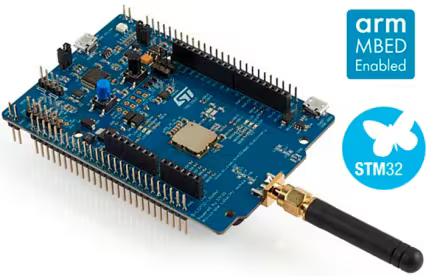
\includegraphics[width=0.5\textwidth]{images/3/loraboard.png}
    \caption{B-L072Z-LRWAN1 LoRa discovery kit}
    \label{fig:bl072}
\end{figure}

It's a development board by STM, integrating a \texttt{STM32L072CZ}\cite{STM32L072CZUltralowpowerArm} arm M0+ processor, that can work at a max clock speed of \texttt{32 MHz}.

The board has pins to connect directly to an Arduino UNO.

Some examples of the different capabilities and peripherals of the board are:
\begin{itemize}
    \item 192KB of flash memory.
    \item 20KB of RAM.
    \item USER and RESET button.
    \item \acrshort{i2c} and \acrshort{uart} connections.
    \item 16 bit timers along with LowPower timers.
    \item Low Power modes.
    \item A SX1276 transceiver that will be used to implement LoraWan communications on the next subject.
\end{itemize}


\subsubsection{Accelerometer}
The accelerometer for this project is the Adafruit breakout board\cite{DownloadsAdafruitMMA8451} for the MMA8451Q\cite{MMA8451Q1a} seen in \autoref{fig:mma}.
\begin{figure}[H]
    \centering
    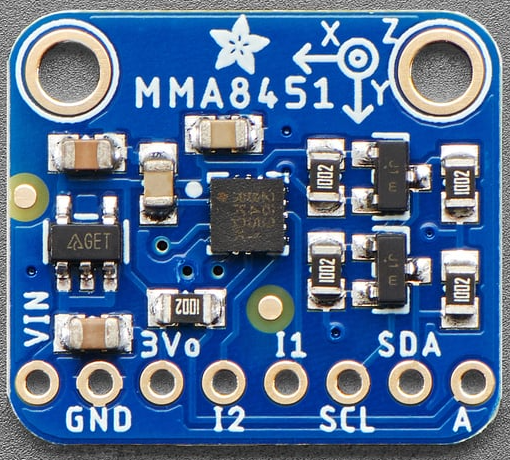
\includegraphics[width=0.3\textwidth]{images/3/mma.png}
    \caption{MMA8451Q by Adafruit}
    \label{fig:mma}
\end{figure}
The MMA8451Q chip by Freescale if the most precise of it's own family, with a triple-axis 14 bit accelerometer. The sensor communicates with the \acrshort{i2c} interface, capable of \texttt{400 kHz}, but as will be seen 
in chapters, the sensor expects a repeated-start communication, this would be a later source for problems.

The chip uses 3.3V, but the Adafruit regulator allows for 5V power supply.

The sensor allows for the configuration of several parameters such as:
\begin{itemize}
    \item Scale of the measurement.
    \item \acrfullr{odr} as low as \texttt{1.56 Hz}.
    \item Power modes.
    \item Interruptions in two pins from situations such as: orientation changes, motion detection, freefall, pulse detection, etc.
\end{itemize}
All this information was taken from the dataset\cite{MMA8451Q1a}.


\subsubsection{Color sensor}
For the analysis of the plant leaves, the TCS34725\cite{TCS34725} in \autoref{fig:TCS34725} is used.
\begin{figure}[H]
    \centering
    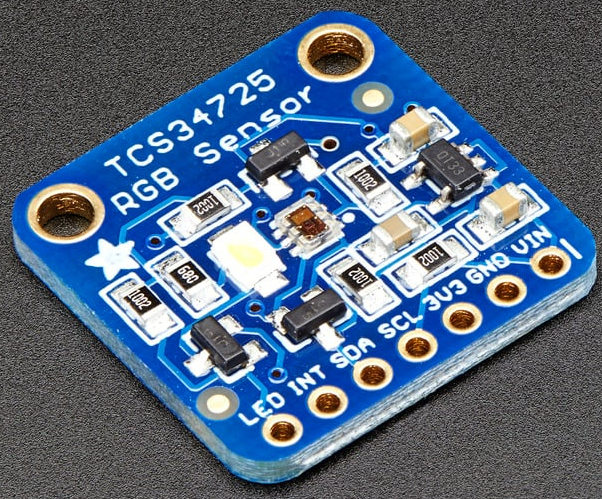
\includegraphics[width=0.3\textwidth]{images/3/color.png}
    \caption{TCS34725 RGB Color sensor by Adafruit}
    \label{fig:TCS34725}
\end{figure}
This chip by \acrfullr{taos} in the 5V compatible breakout board by Adafruit consist on a 3 by 4 photodiode array connected to several integrators that analyze different parts of the visible spectrum. It includes an 
IR blocking filter integrated in the chip that allows for color sensing closer to the vision of humans. Finally, it includes a LED that is driven by the correspondent pin.

It provides readings for clear, red, green and blue values in a 16 bit format. The user can configure things such as:
\begin{itemize}
    \item Integration time.
    \item Wait time between readings.
    \item Interruptions for the clear reading, both in low and high thresholds.
    \item Analog gain.
\end{itemize}

The communication is done with an \acrshort{i2c} interface, capable of \texttt{400 kHz}.

All this information was taken from the dataset\cite{TCS34725}.


\subsubsection{Temperature and Humidity sensor}
The Adafruit Si7021A20\cite{Support_Documents_TechnicalDocs_Si7021A20} in \autoref{fig:Si7021A20} is used.
\begin{figure}[H]
    \centering
    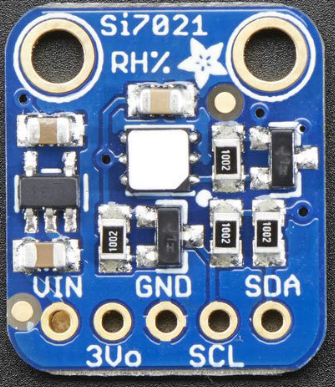
\includegraphics[width=0.3\textwidth]{images/3/th.png}
    \caption{Temperature and Humidity sensor by Adafruit}
    \label{fig:Si7021A20}
\end{figure}
The chip by Silicon Labs communicates with a \acrshort{i2c} interface readings of relative humidity and temperature on-demand. It also allows for the activation of a heating element to remove moisture in the sensor.

All the information was taken from the dataset\cite{Support_Documents_TechnicalDocs_Si7021A20}.
\clearpage
\subsubsection{Positioning module}
The Ultimate GPS v3 by Adafruit\cite{gpsDownloadsAda} in \autoref{fig:gps} is used.
\begin{figure}[H]
    \centering
    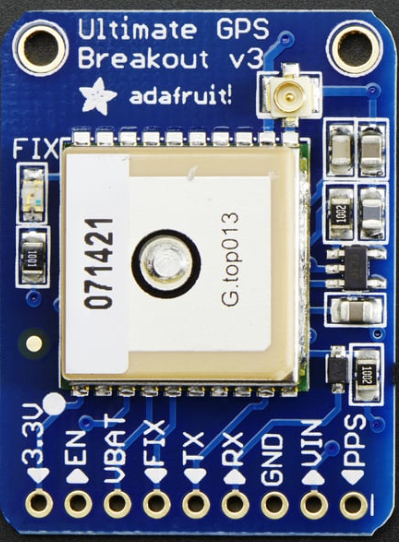
\includegraphics[width=0.3\textwidth]{images/3/gps.png}
    \caption{Ultimate GPS v3 by Adafruit}
    \label{fig:gps}
\end{figure}

This module communicates all the GPS information by an \acrshort{uart} connection. For this, the sensor sends periodic data to the \acrshort{uart} with the \acrfullr{nmea} data format.

This module achieves a level of sensitivity up to \texttt{-165 dBm} with an update rate up to \texttt{10 Hz}.

It includes a PPS output signal for timing applications, and functionalities such as EASY positioning for orbit prediction or AlwaysLocate function to change power consumption in reaction to the needs.

Sadly, the messages and the communication interface to configure this parameters is propietary, and as such, it won't be used in the project.

All the information was taken from the dataset\cite{GlobalTopFGPMMOPA6HDatasheetV0A}.

\subsubsection{Other elements}
The project will also use:
\begin{itemize}
    \item \textbf{SEN-13322 Analog Soil Moisture Sensor}\cite{SparkFunSoilMoisture}: This sensor by SparkFun allows to read the moisture level between the two pads.
    \item \textbf{RGB Led}: A common anode RGB led.
    \item \textbf{Phototransistor}\cite{HW5P1_2015__1_}: This element allows for the reading of the brightness in the environment.
\end{itemize}

\clearpage
\subsection{Block Diagram}
To design the solution, the diagram in \autoref{fig:proposedBlock} identifies the main blocks and hardware interfaces needed. The left side and the GPS include 5V powered elements, and the right side contains 3.3V elements.
\begin{figure}[H]
    \centering
    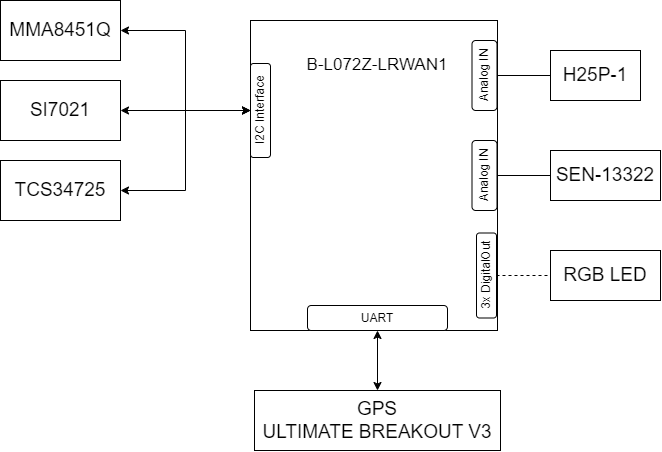
\includegraphics[width=0.6\textwidth]{images/3/General.drawio.png}
    \caption{Block identification for the hardware connections}
    \label{fig:proposedBlock}
\end{figure}

Next, the selection of the connections to the L072CZ were done in the next order: \acrshort{i2c}, \acrshort{uart}, analog connections and finally DigitalOut connections. It is important to note that, as we needed to indicate the working mode with the board leds, we can't 
use the pins connected directly to those elements.
\begin{itemize}
    \item For the I2C, the \acrfullr{mcu} offers 3 options, I2C1,I2C2 and I2C3, being the second one the worst in terms of capabilities.For this system and this use case, I2C1 was selected because, as seen in \autoref{fig:communications}, its the interface with less conflicts.
    \item For the Serial interface to communicate with the GPS, the options are \texttt{USART1}, \texttt{USART2}, \texttt{USART4} and \texttt{USART5}, with the last two having less capabilities. In this case, the L072CZ really only offers the first two, but the \texttt{USART2} 
    is used as a virtual COM port with the ST-Link. The selection was the \texttt{USART1}, also, as can be seen in \autoref{fig:communications}, it has the least conflicts of all.
    \item For the analog sensors, the \texttt{PA\_0} and \texttt{PA\_4} pins were selected, as we only need two Analog IN connections.
\end{itemize}

\begin{figure}[H]
    \centering
    \begin{subfigure}[t]{0.45\textwidth}
        \centering
        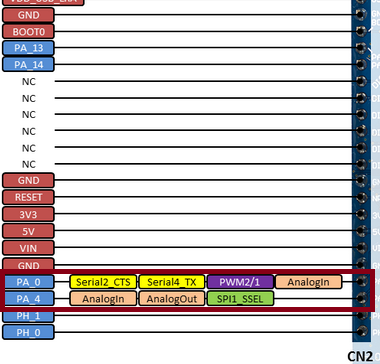
\includegraphics[width=0.66\textwidth]{images/3/Analog.png}
        \caption{Analog selection}
    \end{subfigure}
    \begin{subfigure}[t]{0.45\textwidth}
        \centering
        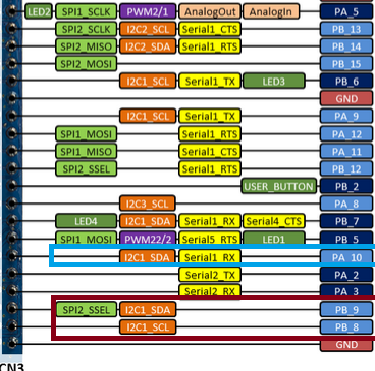
\includegraphics[width=0.66\textwidth]{images/3/I2CSerial.png}
        \caption{I2C and UART selection}
    \end{subfigure}
    \caption{Communication interfaces selection}
    \label{fig:communications}
\end{figure}
\clearpage
At last, the final DigitalOut connections were defined. The final connections for every element are defined in the next tables.
\begin{table}[H]
    \begin{center}
        \begin{tabular}{|p{0.20\textwidth} | p{0.20\textwidth} | p{0.20\textwidth}| p{0.20\textwidth}|}
            \hline
            \textbf{Sensor} & \textbf{Sensor Pin} & \textbf{L072CZ connector} & \textbf{L072CZ Pin name}\\
            \hline
            H25P-1 & SIG & CN2\_24 & PA\_4 \\
            \hline
            SEN-13322 & SIG & CN2\_23 & PA\_0 \\
            \hline
            RGB Led & RED & CN2\_25 & PH\_1 \\
            \hline
            RGB Led & GREEN & CN2\_26 & PH\_0 \\
            \hline
            RGB Led & BLUE & CN2\_10 & PA\_14 \\
            \hline
             & GND & CN2\_17 & GND \\
            \hline
             & VCC & CN2\_19 & +3.3V \\
            \hline
        \end{tabular}
    \end{center}
    \caption{Connections for the 3.3V elements}
    \label{Connections3}
\end{table}
\begin{table}[H]
    \begin{center}
        \begin{tabular}{|p{0.20\textwidth} | p{0.20\textwidth} | p{0.20\textwidth}| p{0.20\textwidth}|}
            \hline
            \textbf{Sensor} & \textbf{Sensor Pin} & \textbf{L072CZ connector} & \textbf{L072CZ Pin name}\\
            \hline
            TCS34725 & LED & CN3\_13 & PA\_9 \\
            \hline
            TCS34725 & INT & CN3\_15 & PA\_11 \\
            \hline
            GPS & SerialTX & CN3\_26 & PA\_10 \\
            \hline
            MMA8451Q & I2 & CN3\_14 & PA\_12 \\
            \hline
             & SCL & CN3\_25 & PB\_8 \\
            \hline
             & SDA & CN3\_24 & PB\_9 \\
            \hline
             & GND & CN3\_26 & GND \\
            \hline
             & VCC & CN2\_20 & +5V \\
            \hline
        \end{tabular} 
    \end{center}
    \caption{Connections for the 5V elements}
    \label{Connections5}
\end{table}

